
% Packages
\documentclass[11pt,a4paper]{article}
\usepackage[utf8]{inputenc}
\usepackage[english]{babel}
\usepackage[T1]{fontenc}
\usepackage{mathptmx}


\usepackage[pdftex]{graphicx}
\usepackage[pdftex,linkcolor=black,pdfborder={0 0 0}]{hyperref}
\usepackage{calc}
\usepackage{enumitem}

% table packages
\usepackage[table, svgnames, dvipsnames]{xcolor}
\usepackage{makecell, cellspace, caption}
\setlength\cellspacetoplimit{3pt}
\setlength\cellspacebottomlimit{3pt}


% citation packages

% \usepackage{biblatex} %Imports biblatex package
\usepackage{csquotes}
\usepackage[backend=biber,natbib=true,style=numeric,sorting=none]{biblatex}

% Import the bibliography file
\addbibresource{refs.bib}


\frenchspacing

% Set linespace
\linespread{1.2}

%margins
\usepackage[a4paper, lmargin=0.1666\paperwidth, rmargin=0.1666\paperwidth, tmargin=0.1111\paperheight, bmargin=0.1111\paperheight]{geometry}

% Tries to remove widows
\usepackage[all]{nowidow}

% Improves typography, load after fontpackage is selected
\usepackage[protrusion=true,expansion=true]{microtype}

\usepackage{lipsum}

% package for authors
\usepackage{authblk}

% add graphics dir
\usepackage{graphicx}
\graphicspath{ {../figures/} }
\usepackage{wrapfig}
\usepackage[export]{adjustbox}

% Begin document
\begin{document}

\begin{titlepage}

    \title{KEGGTOOLS - Toolkit for enrichment and visualization of KEGG pathways}

    \author[1]{Malte Hellmig}

    \author[1, 2]{Prof. Dr. med. Ulf Panzer}
    \author[1, 2]{PD Dr. med. Christian Krebs}

    \affil[1]{\small{\textit{III. Department of Medicine, Division of Translational Immunology, University Medical Center Hamburg-Eppendorf, Hamburg, Germany.}}}
    \affil[2]{\small{\textit{Hamburg Center for Translational Immunology (HCTI), University Medical Center Hamburg-Eppendorf, Hamburg, Germany.}}}
    \date{}
    \clearpage\maketitle
    \thispagestyle{empty}


    \section*{Abstract}

The enlargement of transcriptomic datasets due to high-throughput next-generation
sequencing methods including single cell RNA sequencing, require reproducible and
easy-to-use analysis tools, understandable and expressive visualisations.
A way to address complex information in this field is the enrichment analysis,
which can identify overrepresented classes of genes.
Here, we established KEGGTOOLS, a Python-based package to efficiently compute
and plot enrichment of a
given gene list based on the pathway database of the Kyoto Encyclopedia
of Genes and Genomes. The package is published and freely available on Github:
\mbox{\url{https://github.com/harryhaller001/keggtools}}.

\end{titlepage}

% start new page and set page counter to 1
\newpage
\setcounter{page}{1}

\section*{Introduction}

\subsection*{\textit{Introduction to enrichment analysis}}

In recent years, the field of transcriptomics and genomics has received a strong
boost from the enormous progress in the area of high-throughput sequencing. This
development has been made possible in particular by the technology of next-generation
sequencing (NGS), through which large amounts of genetic information can now be
determined in a very short time and - compared to earlier sequencing methods, such
as Sanger's sequencing method - much more cost-efficiently. However,
since these methods output a large amount of information, the analysis and visualization of this
data has become crucial. The "Gene Ontology Term" analysis, for example, offers the
possibility to assign genes to hierarchically organized domains, so-called "Gene
Ontology Terms" (in short GO terms)\cite{goterm}. In the process of GO term enrichment,
the intersection of a list of analyzed genes with the genes assigned to a GO term is
formed in order to draw conclusions about the change in certain biological processes.
A popular tool for this is the Python library "goatools", that has been cited
already over 200 times\cite{goatools}.


\subsection*{\textit{Structure of KEGG database}}

The Kyoto Encyclopedia of Genes and Genomes (KEGG) was established in 1995 and is a
database of genetic information, biomolecules, metabolic pathways and signaling
pathways for various organisms \cite{kegg1,kegg2}. It was developed by the Kyoto Bioinformatics
Center in collaboration with the "Human Genome Center" in Tokyo. This database not only
contains information about genes and molecules, but also organizes them according to
interaction pathways, the so-called "KEGG pathways" \cite{kegg2}. The data is presented
human-readable on their website (\mbox{\url{https://www.genome.jp/kegg/}}), but is also implemented
in machine-readable form via a public web-based application programming interface (API) in the
style of a representational state transfer (available at \mbox{\url{http://rest.kegg.jp}}).
% The data is also freely accessible to anyone.
The KEGG database offers a large number of
datasets and subordinate databases, but only the signaling pathway and compound database is relevant for this work.
% Since this work deals with the analysis of
% transcriptome data, only the gene, component, and signal pathway databases are relevant
% for this work.

\subsection*{\textit{Aim and functionality of KEGGTOOLS}}

First, this work addresses the high complexity and diversity of the KEGG database
and tries to reduce the effort to use this data source. The KEGGTOOLS package acts
as middleware between analysis and the KEGG database. It solves requests to the API
endpoint, manages cache to reduce bandwidth and latency. Moreover, it parses predefined pathways in
an object-relational style to maintain all the information received by the original
source. Second, this package is designed to perform specific analysis and generate appropriate visualisation. Genes
found in previous analyses can be imported in this software and enriched for sets
of KEGG pathways. Additionally resulting pathways of enrichment analysis can be
visualised with custom overlays, for example results of previously performed differential
expression analysis.


\section*{Results}

\subsection*{\textit{Exemplary analysis of the PBMC3K single-cell RNA dataset}}

To demonstrate the capabilities of the package KEGGTOOLS, the PBMC3K dataset was
used \cite{pbmc3k}. This single cell RNA dataset consists of approximately 3.000 peripheral
blood mononuclear cells (“PBMC”) from a healthy donor and is commonly used for demonstration purposes.
Since the preprocessing of this sample is already described in great detail \cite{seurat,scanpy},
an already published analysis procedure was used. The published analysis reveals seven
different cell types (Figure 2), but in the following analysis, the population identified
as natural killer cells (“NK” cells) was focused on exclusively. This cluster showed
strong upregulation of granzyme B, granzyme A, granulysin and natural killer cell granule
protein 7 in the differential expression analysis (Table 1). All of these genes have
been described previously as common marker genes for natural killer cells \cite{nk-marker-1,nk-marker-2,nk-marker-3}.
For the 100 differentially expressed genes with the highest significance in the NK cell
cluster the enrichment analysis with KEGGTOOLS was performed. To reduce the number of
pathways for the enrichment analysis only immunological relevant pathways were selected (20 pathways out of a total of 332).
The analysis with KEGGTOOLS highlighted the pathway “Natural killer cell mediated cytotoxicity”
(hsa:04650) as significantly enriched in the NK cell cluster (Table 2). Differentially expressed genes were then
combined with the pathway graphs (Figure 5). By combining the color gradient with the
individual genes of the pathway, it is not only possible to visualize the interactions
between the genes in general, but also to intuitively highlight the significance of
individual genes. Thus, in this exemplary analysis, the pathway created shows the particular
importance of granzyme B as well as an increase in downstream signaling of tyrosine
tinase FYN and LCK.


\section*{Material and Methods}


\subsection*{\textit{IO structure and caching}}


The KEGG pathways are uniquely identifiable via a unique organism identifier as a
three-letter code (for example “mmu” for mus musculus) as well as a KEGG pathway
identifier - a five-digit number - that is unique for the respective organism.
Using this information, the data of a pathway can be downloaded in KGML format,
the so-called KEGG Markup Language (KGML), from the API. To receive the collection
of all pathways the KEGG API provides
an endpoint to list all available pathways for a given organism. This list is then
used to search and download pathways. In order to make the most efficient use of the
data retrieved from KEGG database, KEGGTOOLS library uses a caching. After retrieval,
the data is stored locally in the KEGGTOOLS library folder and the local copy is made
available when a new request is made. This keeps traffic and the load on the API of
the KEGG database low and increases the speed when the analyses are repeated.
Before performing an enrichment analysis, the KGML files of all KEGG pathways
associated with the organism are first loaded into the memory. The list of all
paths of an organism with names and unique identifiers are retrieved from the KEGG
API. If a KEGG pathway is not included as a local copy, the KGML file is downloaded
and saved. Subsequently, all pathways of the organism are converted into an object-relational
form and stored in the memory. In order to be able to represent the complete
pathway, the names of the compounds, which are deposited in the KGML format
only as identifiers, are loaded. These compounds have a unique identifier
and are common across all organizations. For faster accessibility of this list
this is stored also locally in the cache in serialized form.


\subsection*{\textit{Parsing of KEGG pathways}}

The programming interface for the signal paths uses a format developed for the KEGG
database for the transmission of the data.
This file format with the file extension "*.kgml" is based on the standard of the
Extensible Markup Language (XML) and encodes the genes and components of a signal
or metabolic pathway. In addition, the relationships of the individual components of
a pathway as well as additional attributes, such as the name, uniform identifiers and
cross-references to the KEGG database, are transmitted in this format (Table 2).
The different elements of this format are also in a hierarchical relationship to each
other (See: Appendix Figure 1), with the element "pathway" always forming the root
element (so-called "root"). The element "entry" stores the entries in the pathway,
such as genes, while the element "relation" characterizes the relationship between two
entries in more detail. The properties are stored as a key-value combination in the
standard XML format within the elements.


\subsection*{\textit{Enrichment and statistical analysis}}

The enrichment analysis is an iteration through all input genes as a list of NCBI gene database identifier, the so-called Entrez
identifiers \cite{entrez}, within an iteration through all genes of all pathways belonging to the
organism. A match of the Entrez identifier between the examined gene and a gene of
a KEGG pathway is counted as a hit. For each pathway, hits are stored and pathway-specific
hits are summarized at the end of the analysis. In the final summary of the enrichment
analysis, the name and identifier of the investigated KEGG pathway, hits per KEGG pathway,
the total number of genes of the pathway, the list of Entrez identifiers of the found
genes, and the p-value are stored as character-separated values (CSV). For statistical
analysis and the determination of the p-value within the enrichment analysis, the
Fisher's exact test is used. The null hypothesis for an analysis result of a single
pathway A with the list of genes B found is assumed to be: "There is no association
between the genes B examined and the genes associated with KEGG pathway A”. The p-value
is determined by the corresponding contingency table. In order to be able to limit the
results of the enrichment analysis due to the large number of KEGG pathways that can be
examined, it is possible to limit the results after the analysis by forming subgroups.
For example, a list of KEGG pathway identifiers can be specified and thus limit
the analysis to relevant pathways.
% The KEGG website provides a list of pathways grouped
% by corresponding domains, which does not have a corresponding  API endpoint
% (See \mbox{\url{https://www.genome.jp/kegg/pathway.html}}).


\subsection*{\textit{Reproducibility and best practices}}

The KEGGTOOLS package follows several best practices to make a valuable contribution
to the science and open-source community. The source code together with all analyses
which are part of this publication are publicly available via Github. The package also
includes automated tools for Continuous Integration/Continuous Delivery (CI/CD).
This includes static code analysis, linting and unittest which are all integrated as
automated tasks in the repository. This automation should facilitate future development,
also with other collaborators.


\section*{Discussion}

\subsection*{\textit{Achievement of KEGGTOOLS}}

The KEGGTOOLS package provides an easy-to-use package to download and process information from
the KEGG database. The package internal caching reduces internet traffic and enables faster
analysis. Compared to other enrichment analysis datasets, such as GO terms \cite{goterm}, the KEGG pathways
include the interactions of genes and components. This interactional information allows for
improved visualization of the pathways, which would not be possible with other enrichment
datasets.

\subsection*{\textit{Informational value of KEGGTOOLS analysis}}

KEGG pathways often consist of gene entries which are not directly associated with an
investigened cell itself. The pathway “Natural killer cell mediated cytotoxicity” examined
in the example enrichment analysis also includes genes with which NK cells commonly
interact, like genes of the HLA family. This has the potential problem of a statistical
bias within the enrichment analysis, because the total number of genes in a pathway
increases with no underlying biological basis. An issue which is not present in GO
term enrichment analysis, since GO terms form distinct and hierarchical semantic
units\cite{goterm}. Despite this problem, the possibility of visualization by KEGGTOOLS
has the advantage that not only hierarchical but also interactional information can
be displayed.

\subsection*{\textit{Known issues of the KEGGTOOLS package}}

When running pathway enrichment analyses with a large amount of pathways, it is
possible to create a timeout error. This happens when requesting too many resources
from KEGG database API and the backend rejecting further requests. To solve this
potential issue, this package provides an external link to download all human and
murine KGML files as compressed archive. It is important to note that these data may
not be up to date. Another way to combat this problem is to use a request sleep, which
can be specified when initializing a KEGGTOOLS resolver instance.


% Citations
\newpage

\printbibliography %Prints bibliography

\newpage


% figure of KEGG database structure
% \begin{wrapfigure}{l}{0.5\textwidth}

%     % 1142x1858 px
%     \centering{
%         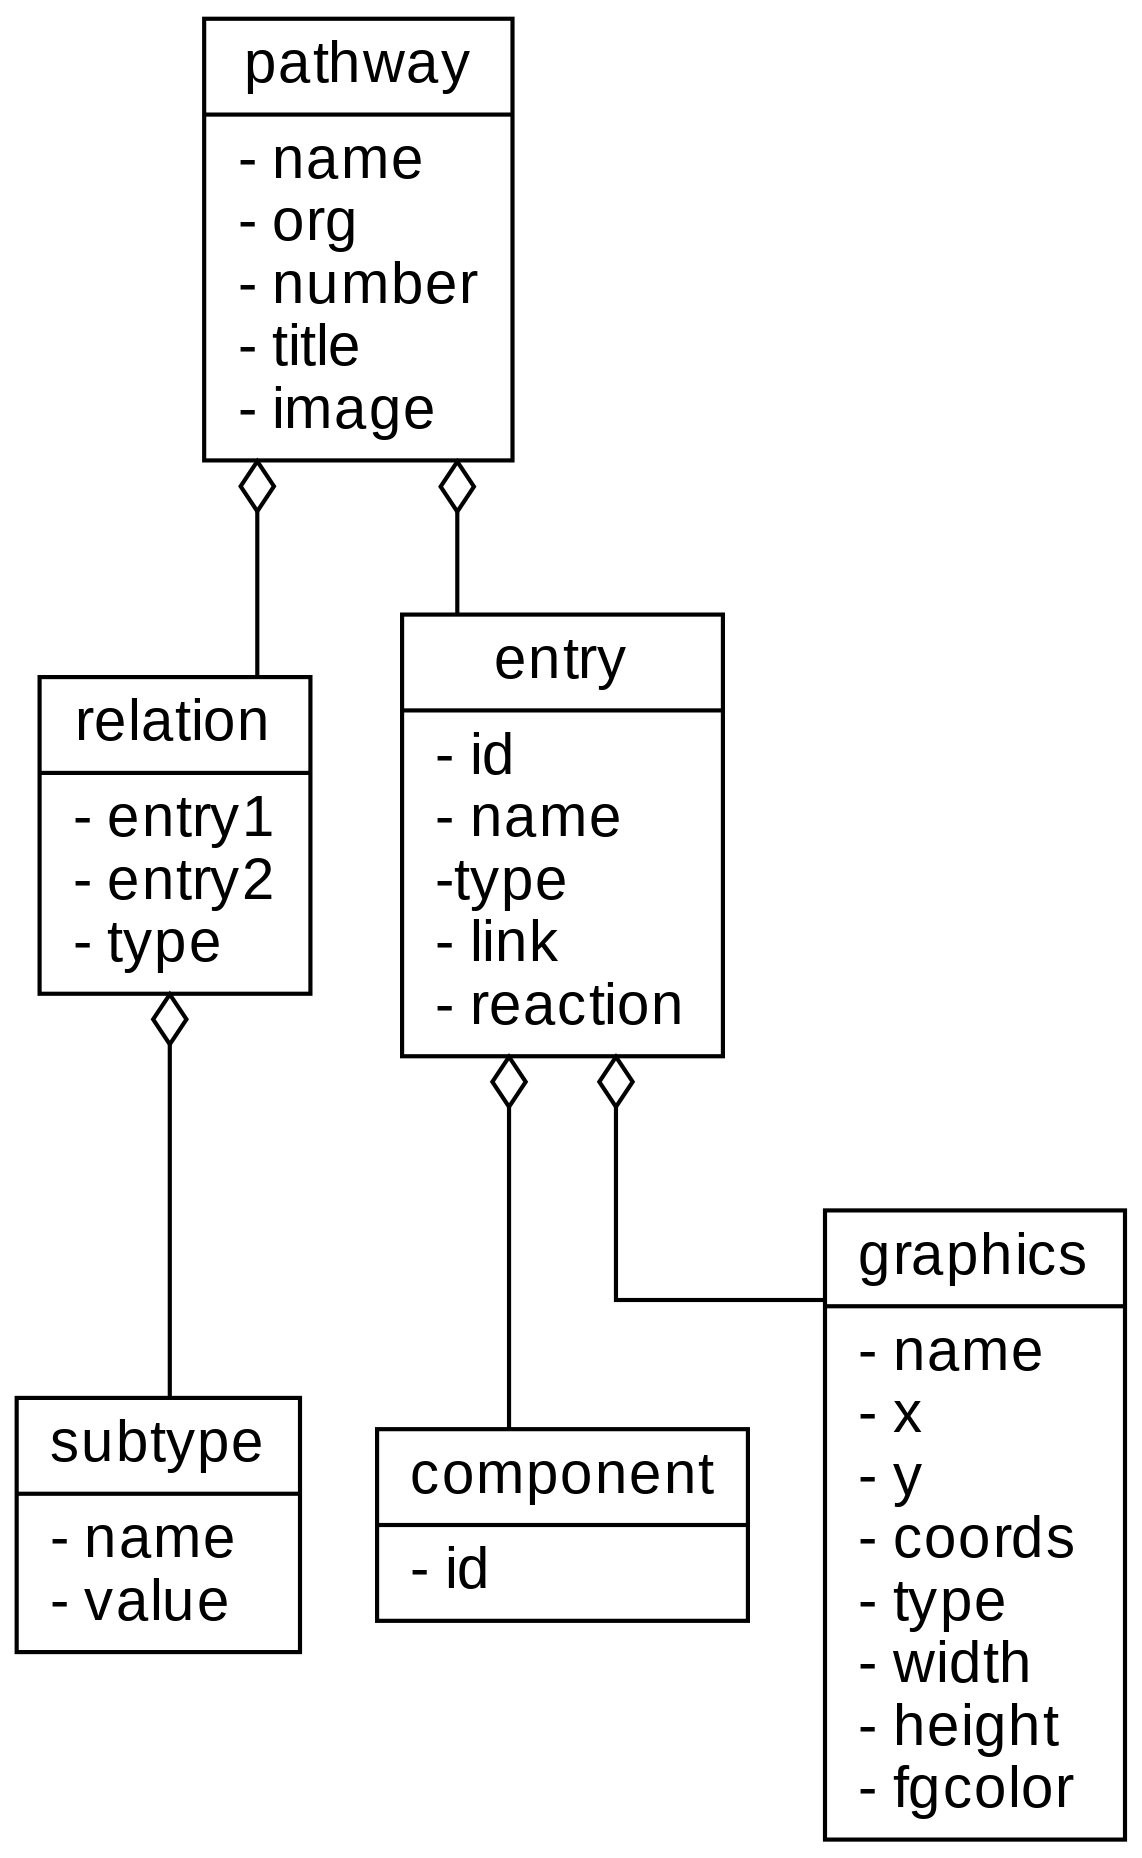
\includegraphics[width=5cm]{figure1.png}
%     }

%     \caption{Object structure of KEGG database models}
% \end{wrapfigure}

% figure of KEGG database structure
\begin{figure}

    % 1142x1858 px
    \centering{
        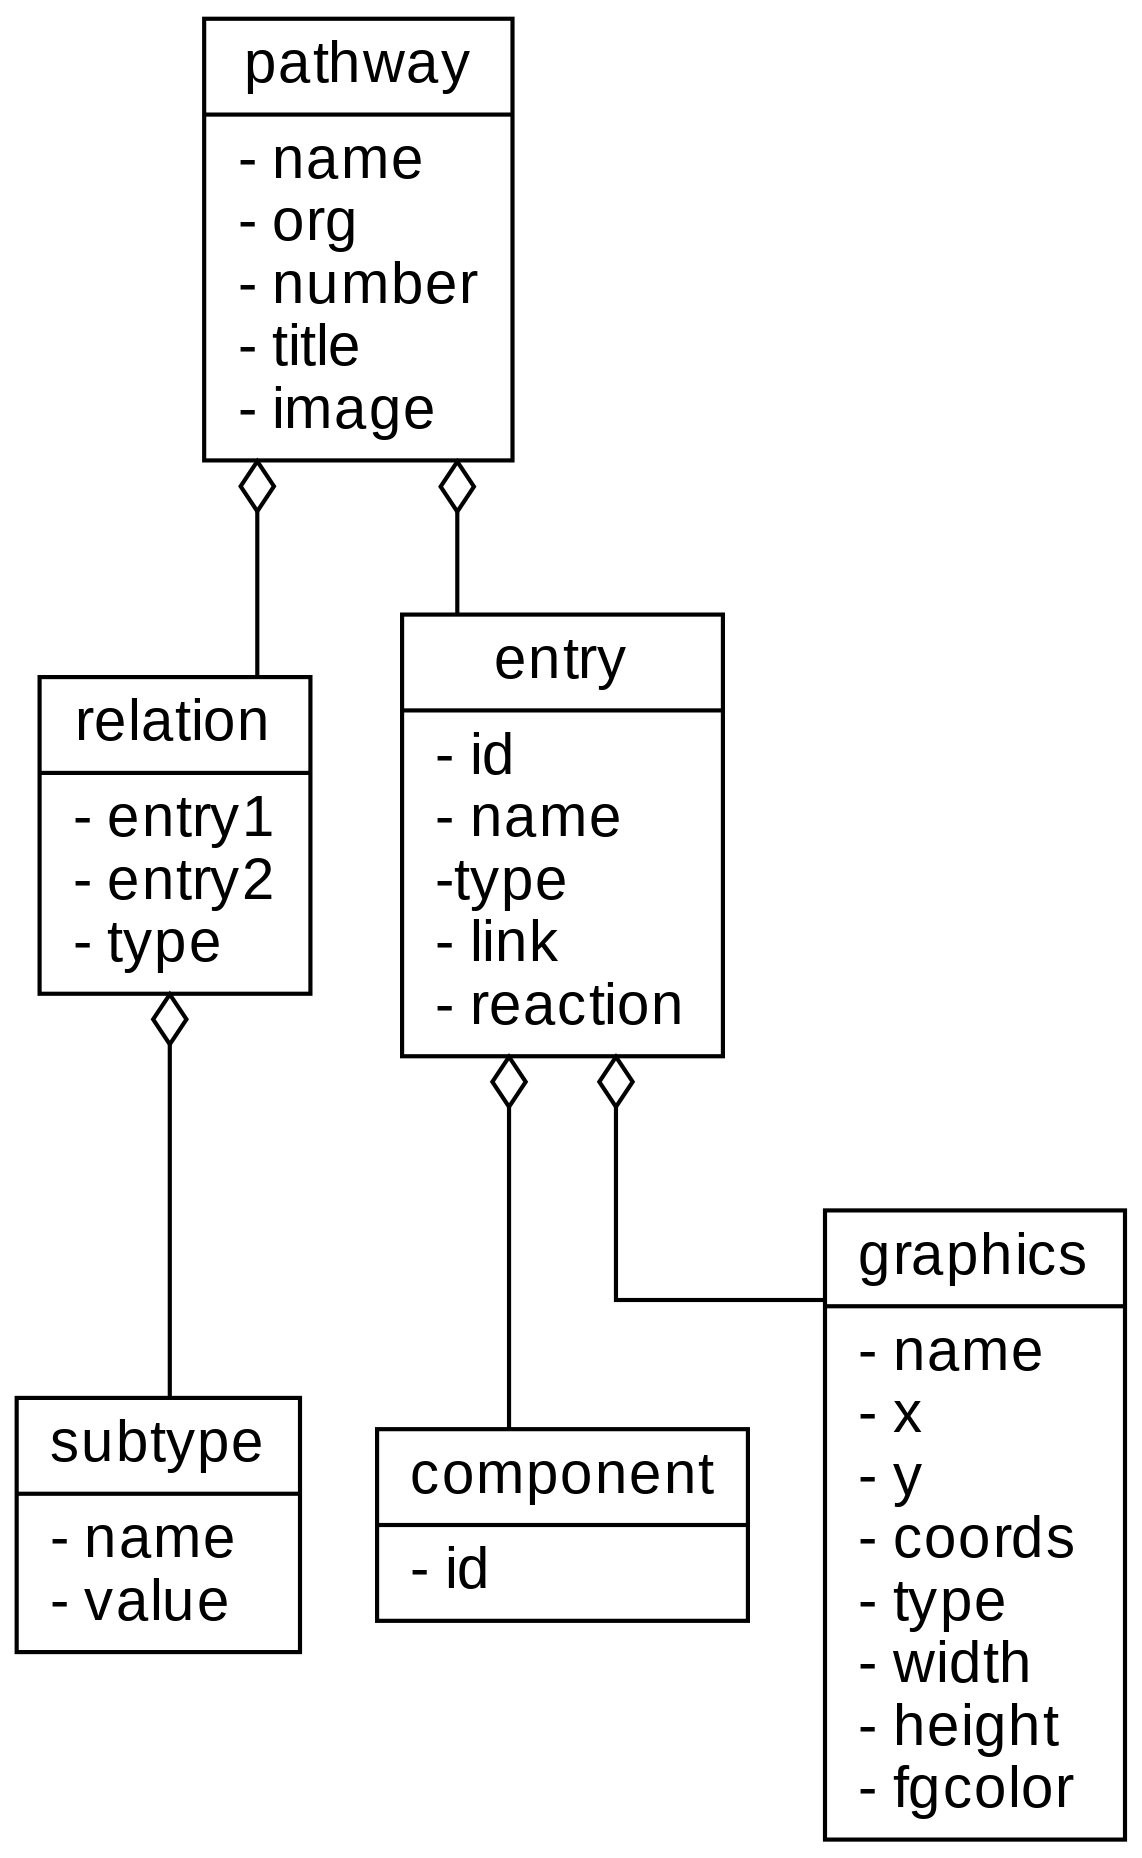
\includegraphics[width=5cm]{figure1.png}
    }

    \caption{Object structure of KEGG database models.}
\end{figure}


% Figure of single cell analysis
\begin{figure}

    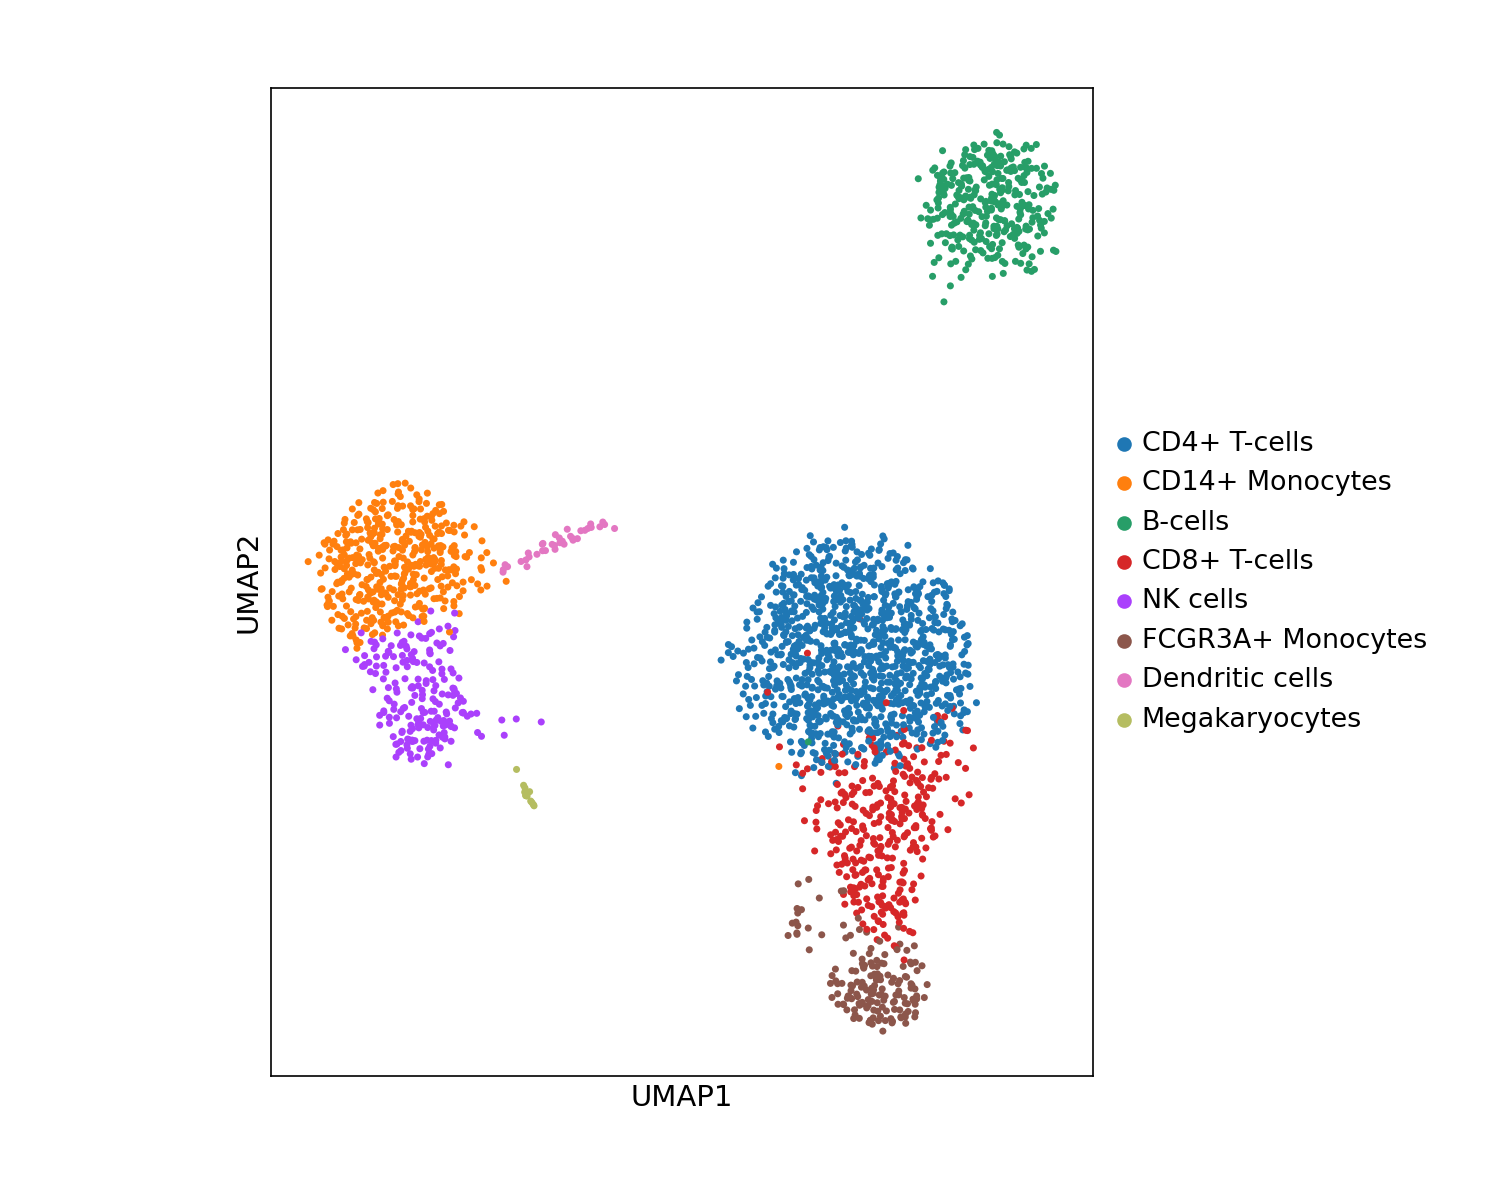
\includegraphics[width=0.5\textwidth, valign=t]{figure2.png}
    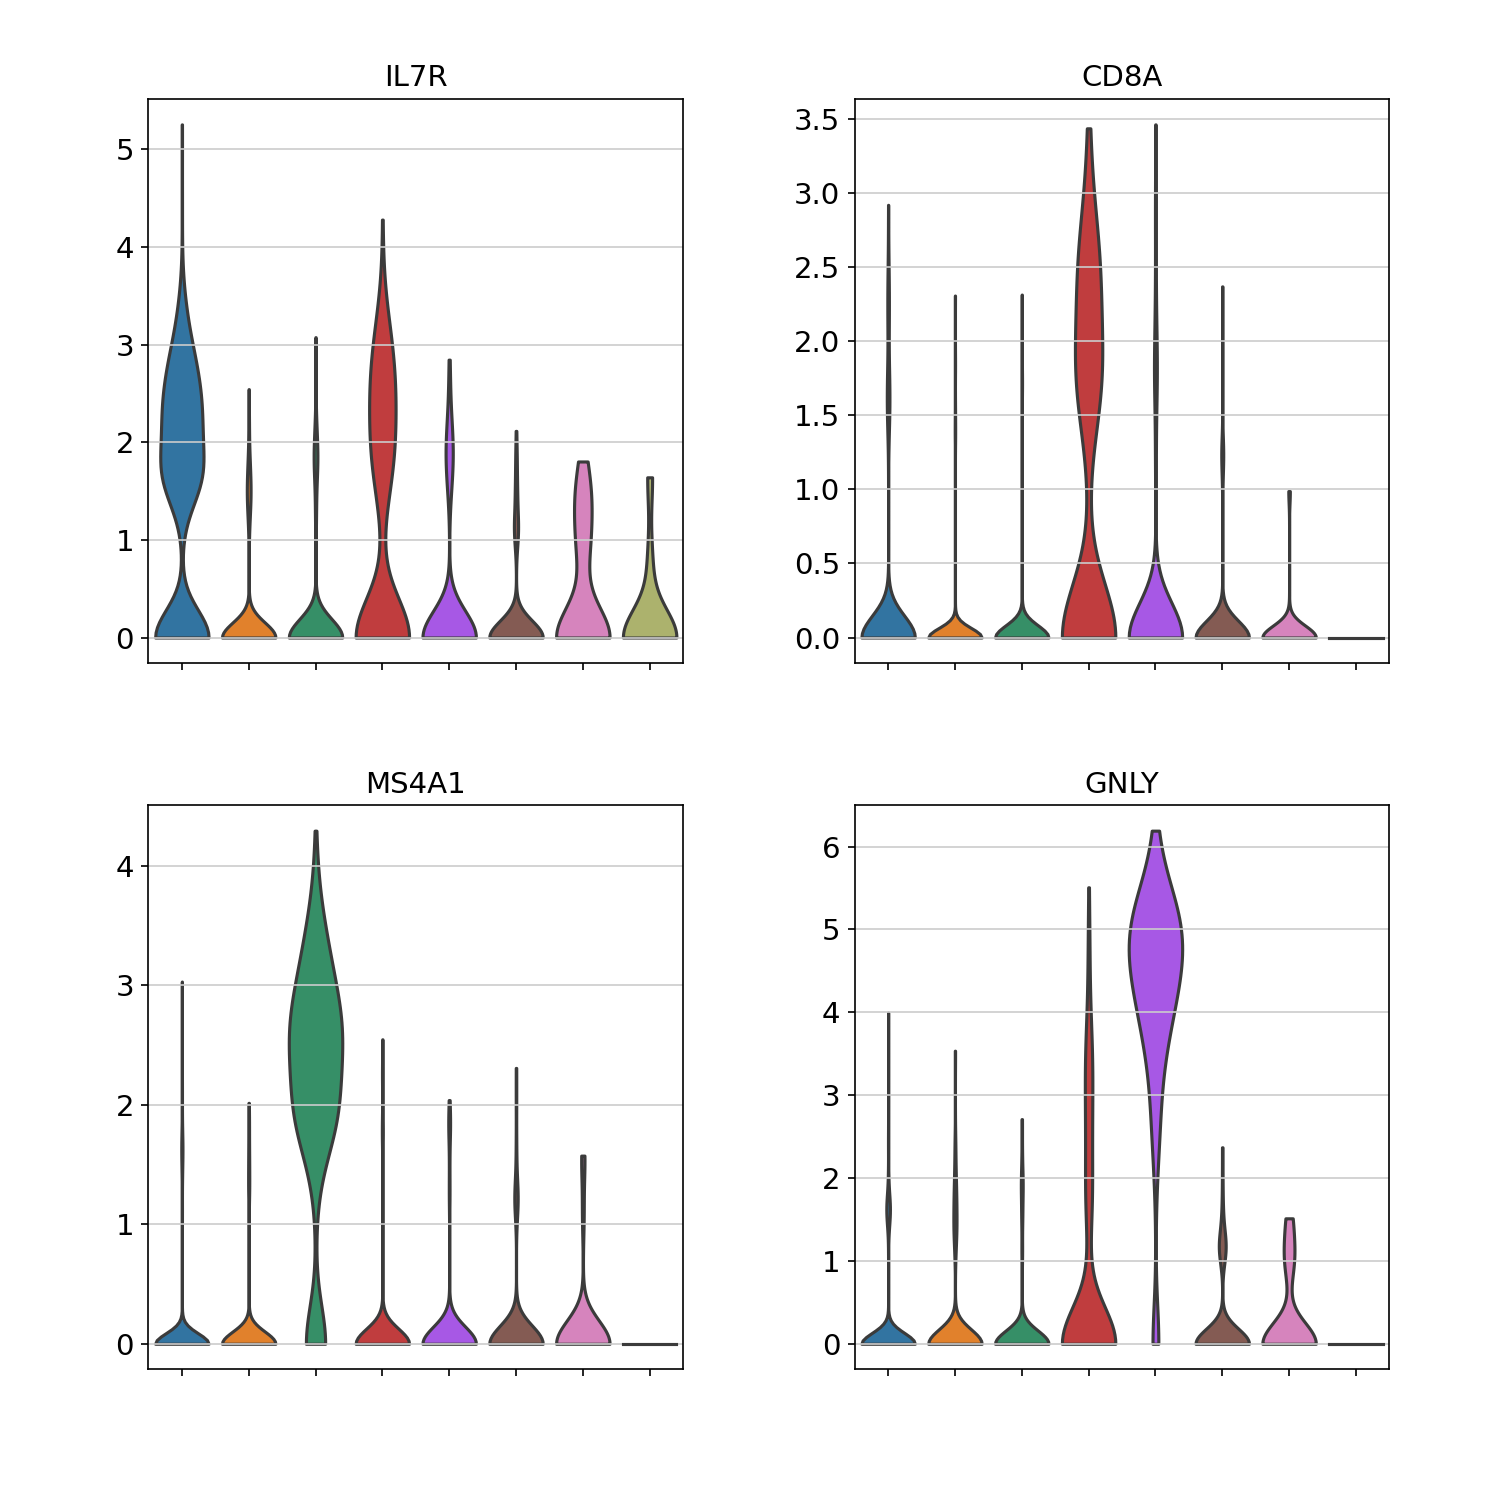
\includegraphics[width=0.5\textwidth, valign=t]{figure3.png}

    \caption{Analysis of the single cell RNA dataset PBMC3K. It show the cell distribution in the UMAP space with
    cluster annotation (left) and identified marker genes (right).
    }
\end{figure}


% Figure for enrichment analysis result

\begin{figure}
    \centering{
        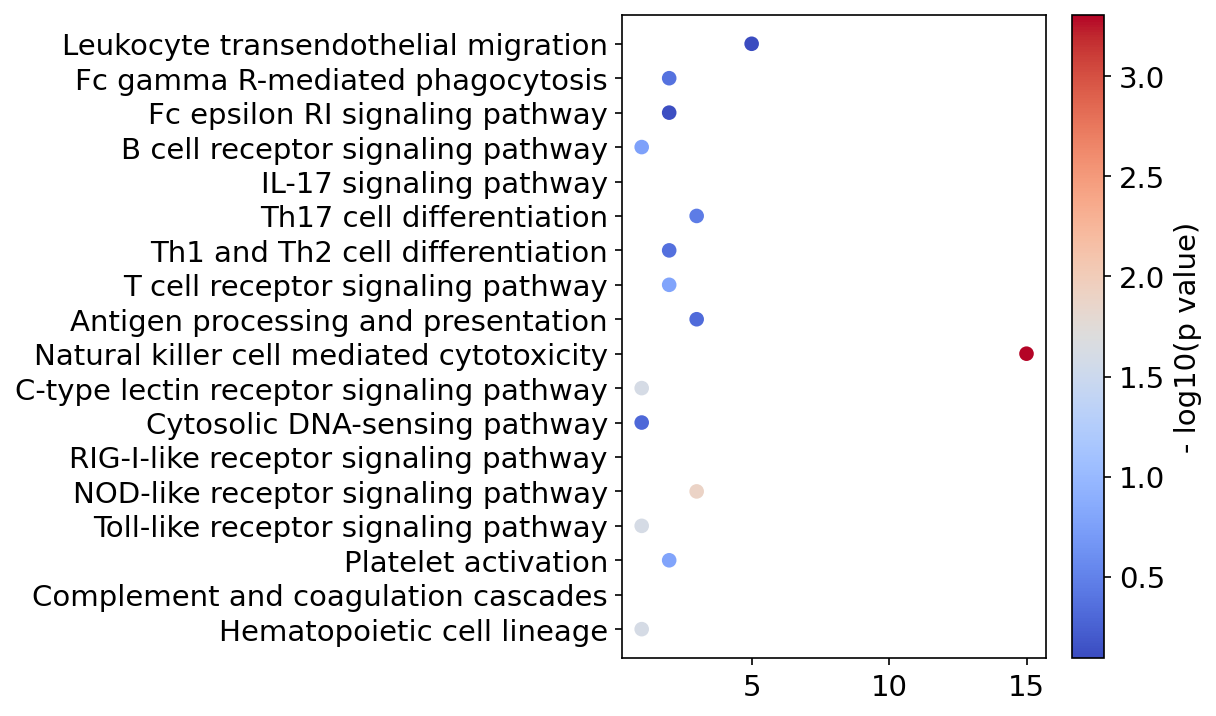
\includegraphics[width=10cm]{figure4.png}
    }

    \caption{Result of KEGGTOOLS analysis showed a significant enrichment of the KEGG pathway "Natural killer cell
    mediated cytotoxicity".}
\end{figure}

\begin{figure}
    \centering{
        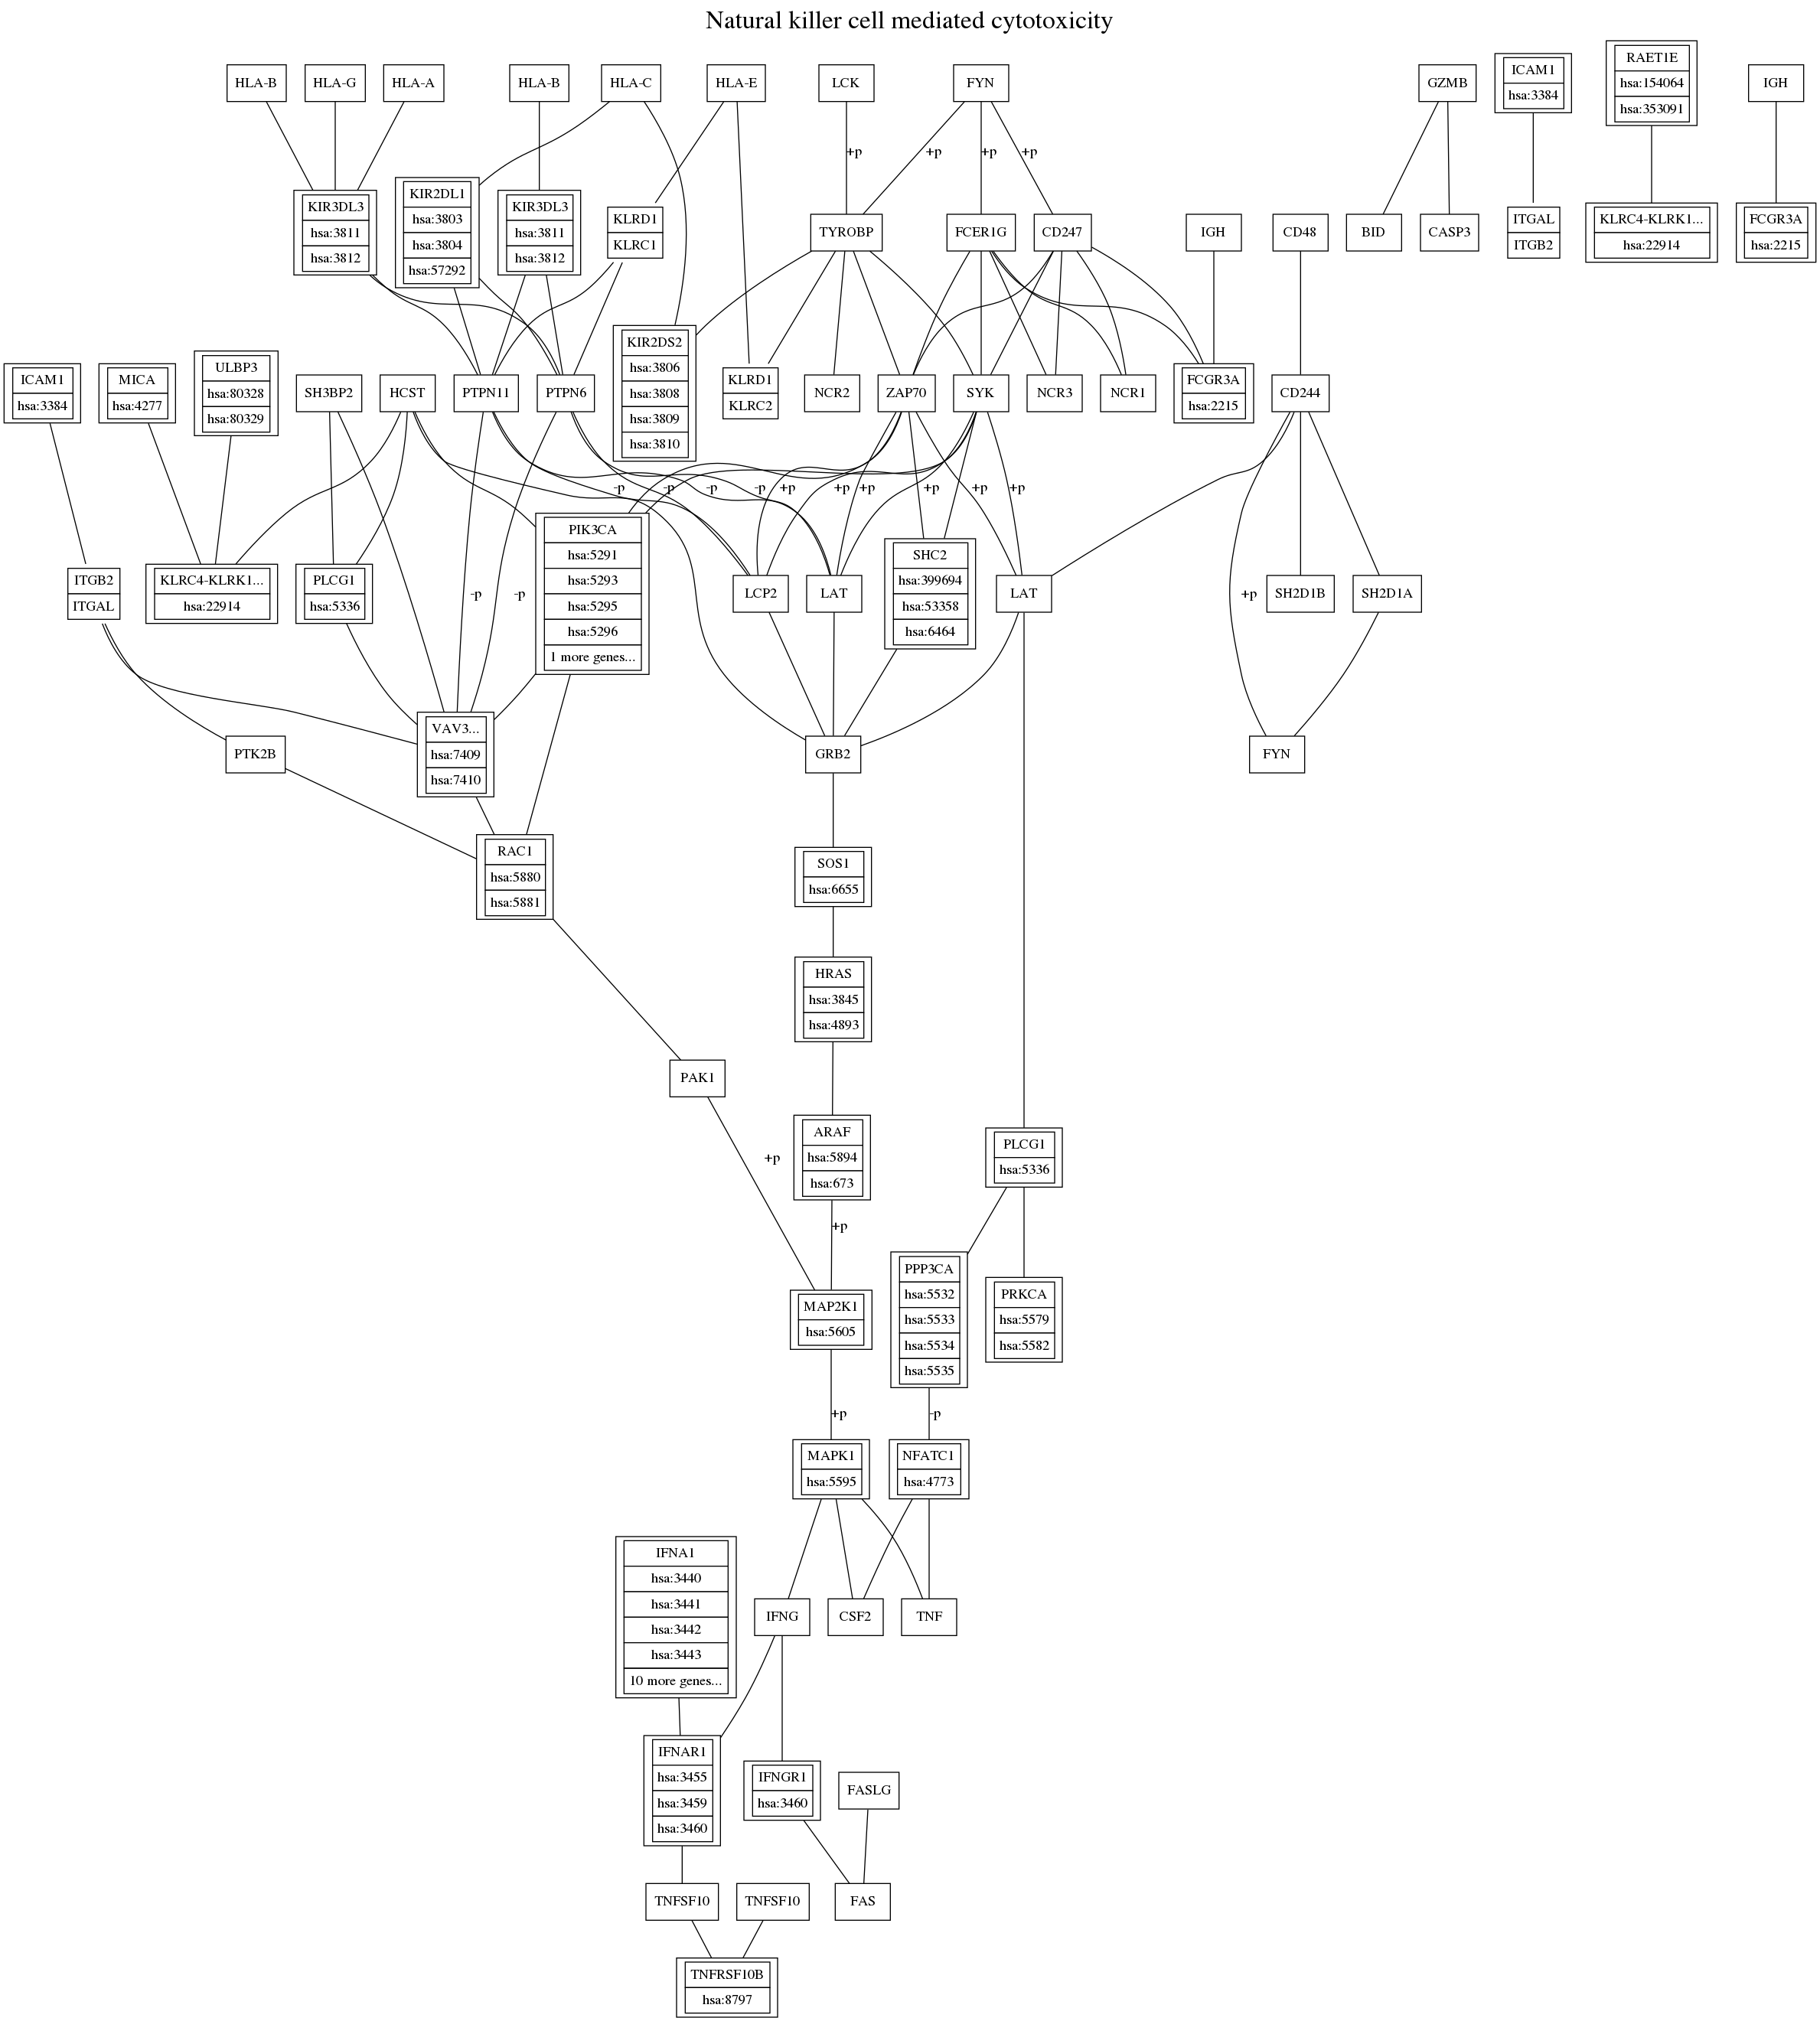
\includegraphics[width=\textwidth]{figure5.png}
    }

    \caption{Rendering of the KEGG pathway "Natural killer cell mediated cytotoxicity" with an color-coded overlay of
    the corresponding differential expression.}
\end{figure}

%% Tables


\begin{table}
    \begin{tabular}{ | l | l | l | l |}
    \hline
    \rowcolor{Gainsboro!60}

    Gene & Symbol & \makecell{p value \\ (abjusted)} & log fold expression  \\ \hline
    Natural killer cell granule protein 7 & NKG7 & 5.92e-92 & 6.88 \\ \hline
    Granulysin & GNLY & 2.38e-84 & 7.83  \\ \hline
    Granzyme B & GZMB & 2.38e-84 & 7.67 \\ \hline
    Cathepsin W & CTSW & 4.12e-83 & 4.83 \\ \hline
    Perforin 1 & PRF1 & 1.39e-81 & 6.32 \\ \hline
    Granzyme A & GZMA & 2.14e-74 & 5.31 \\ \hline
    Cystatin F & CST7 & 4.35e-74 & 5.31 \\ \hline
    Major Histocompatibility Complex, Class I, C & HLA-C & 4.73e-71 & 1.47 \\ \hline

    \end{tabular}

    \caption{Top differentially expressed genes of the NK cells cluster (selected according to p value)}
\end{table}


\begin{table}
    \begin{tabular}{ | l | l | l | l |}
    \hline
    \rowcolor{Gainsboro!60}

    Pathway name & KEGG Id & \makecell{p value \\ (abjusted)} & total hits  \\ \hline

    Hematopoietic cell lineage & 04640 & \textbf{0.024*} & 1/67 \\ \hline
    Complement and coagulation cascades & 04610 & - & 0/62 \\ \hline
    Platelet activation & 04611 & 0.163 & 2/64 \\ \hline
    Toll-like receptor signaling pathway & 04620 & \textbf{0.024*} & 1/67 \\ \hline
    NOD-like receptor signaling pathway & 04621 & \textbf{0.013*} & 3/113 \\ \hline

    RIG-I-like receptor signaling pathway & 04622 & - & 0/50 \\ \hline
    Cytosolic DNA-sensing pathway & 04623 & 0.505 & 1/29 \\ \hline
    C-type lectin receptor signaling pathway & 04625 & \textbf{0.024*} & 1/67 \\ \hline
    Natural killer cell mediated cytotoxicity & 04650 & \textbf{0.0005***} & 15/70 \\ \hline
    Antigen processing and presentation & 04612 & 0.469 & 3/25 \\ \hline
    T cell receptor signaling pathway & 04660 & 0.161 & 2/63 \\ \hline
    Th1 and Th2 cell differentiation & 04658 & 0.429 & 2/49 \\ \hline
    Th17 cell differentiation & 04659 & 0.356 & 3/62 \\ \hline
    IL-17 signaling pathway & 04657 & - & 0/70 \\ \hline
    B cell receptor signaling pathway & 04662 & 0.169 & 1/44 \\ \hline
    Fc epsilon RI signaling pathway & 04664 & 0.766 & 2/38 \\ \hline
    Fc gamma R-mediated phagocytosis & 04666 & 0.422 & 2/46 \\ \hline
    Leukocyte transendothelial migration & 04670 & 0.809 & 5/56 \\ \hline
    Intestinal immune network for IgA production & 04672 & - & 0/33  \\ \hline
    Chemokine signaling pathway & 04062 & - & 0/52 \\ \hline

    \end{tabular}

    \caption{Results of KEGGTOOLS enrichment analysis performed with differential expressing of NK
    cells for immunological KEGG pathways. For determination of the p value the Fisher exact test was used. (p < 0.05 * p < 0.001 ***)}
\end{table}

\end{document}

